\documentclass[usenames,dvipsnames]{beamer}

\usepackage[utf8]{inputenc}
\usepackage[francais]{babel}
\usepackage{wrapfig}
\usepackage{amsmath}% http://ctan.org/pkg/amsmath
\usepackage{graphicx}

\usepackage{multirow}

\usepackage{sansmathaccent}
\pdfmapfile{+sansmathaccent.map}
\usepackage{tikz}
\usepackage{verbatim}

% \setbeamertemplate{caption}{\raggedright\insertcaption\par}
\beamertemplatenavigationsymbolsempty
\setbeamertemplate{caption}[numbered]
\setbeamertemplate{footline}[frame number]

\usetheme{Singapore}

\title{Détection d'anomalies de classification dans l'IoT via Machine Learning}
\author{Antoine Urban, Yohan Chalier}
\institute{Projet de filière SR2I \\ Télécom ParisTech}

\begin{document}

\begin{frame}
\titlepage
\end{frame}

\section{Introduction}

\begin{frame}{Introduction}
La détection d'obstacles: un enjeu de sécurité !
\begin{figure}
\centering
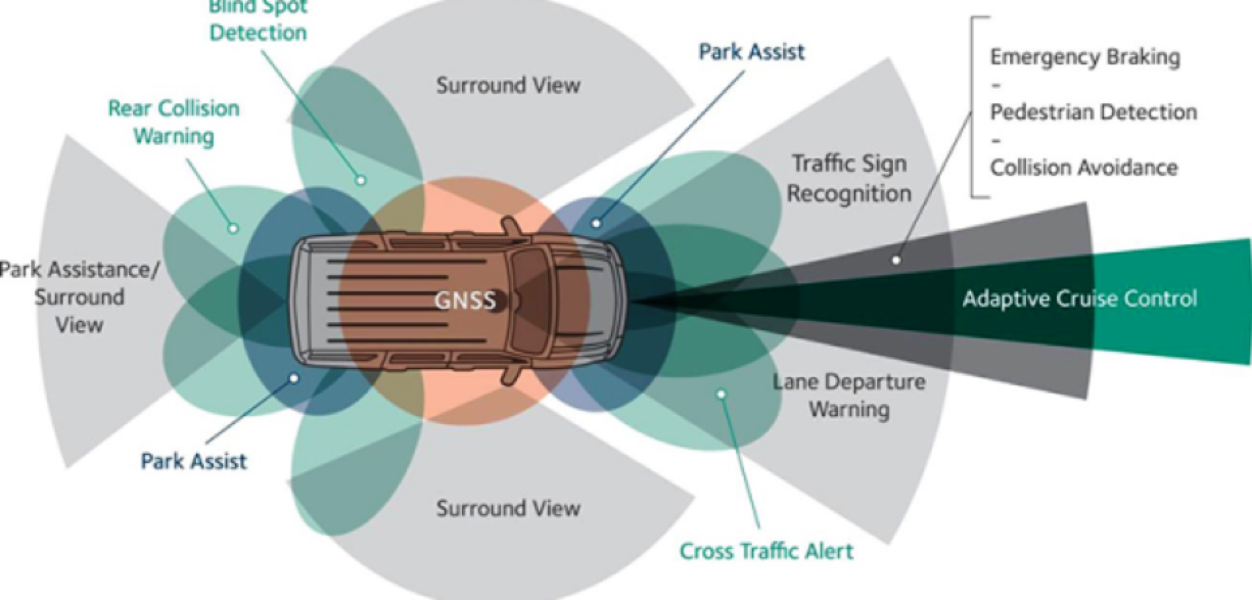
\includegraphics[width=.8\textwidth]{img/sensors.png}
\caption{Fonctions automatisées nécessitant un ou des capteur(s)}
\end{figure}
\end{frame}

\begin{frame}{Attaques potentielles}

\begin{columns}

\begin{column}{0.5\textwidth}
\begin{figure}
\centering
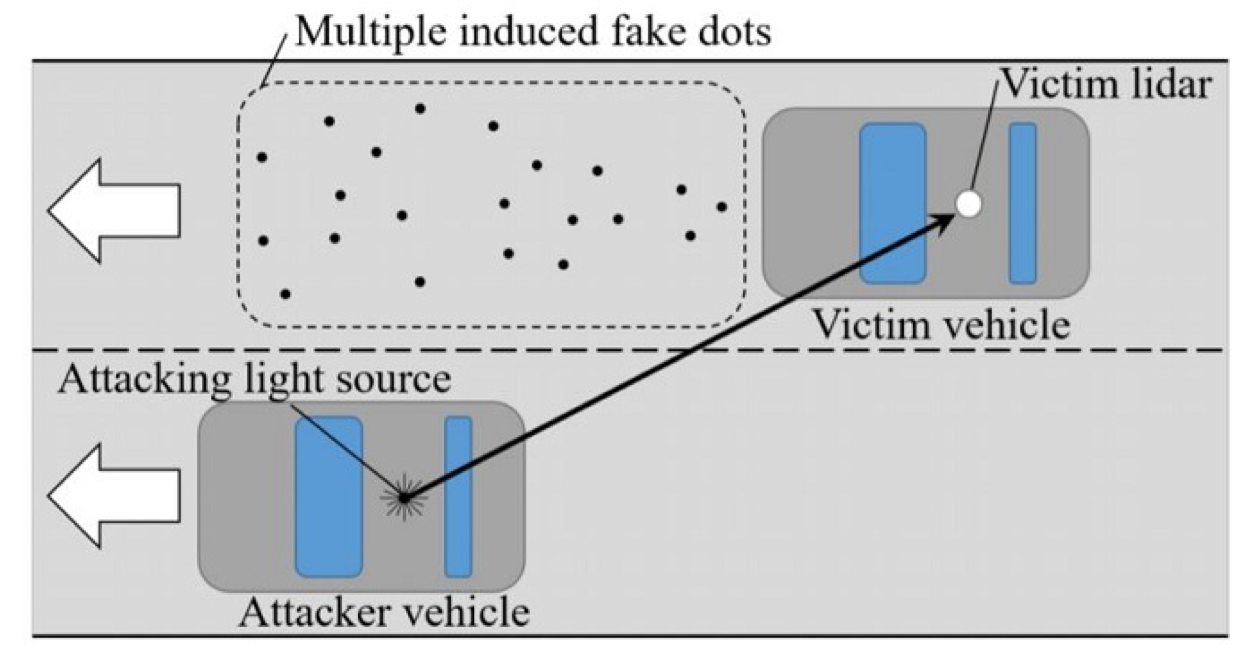
\includegraphics[width=\textwidth]{img/blinding.png}
\caption{Attaque par aveuglement des capteurs}
\end{figure}
\end{column}

\begin{column}{0.5\textwidth}
\begin{figure}
\centering
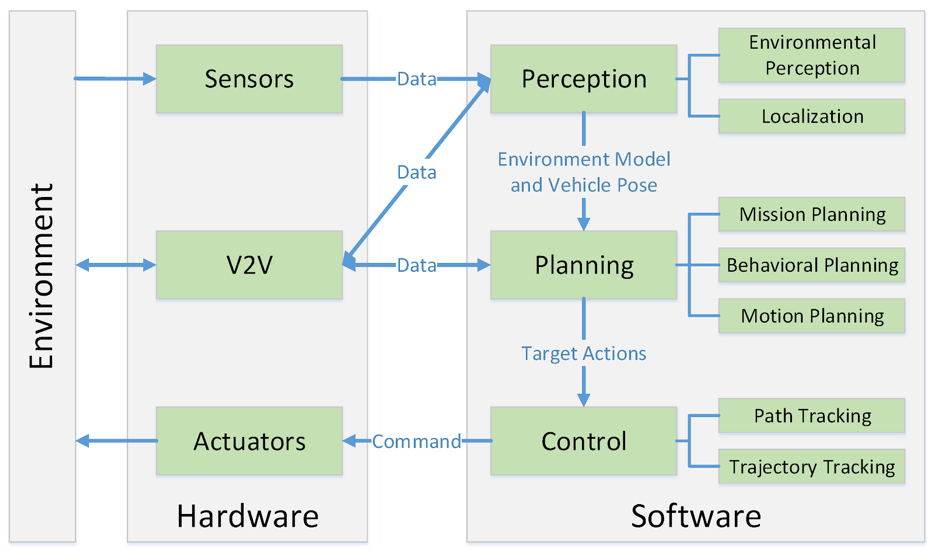
\includegraphics[width=\textwidth]{img/data_flow.png}
\caption{Attaque par modification}
\end{figure}
\end{column}

\end{columns}

\end{frame}


\begin{frame}{Objectifs}
Proposition d'un modèle de classification multi-classes en réalisant un classeur à partir d'un algorithme d'apprentissage supervisé.
\end{frame}

\begin{frame}{Système de classification}
\begin{figure}
\centering
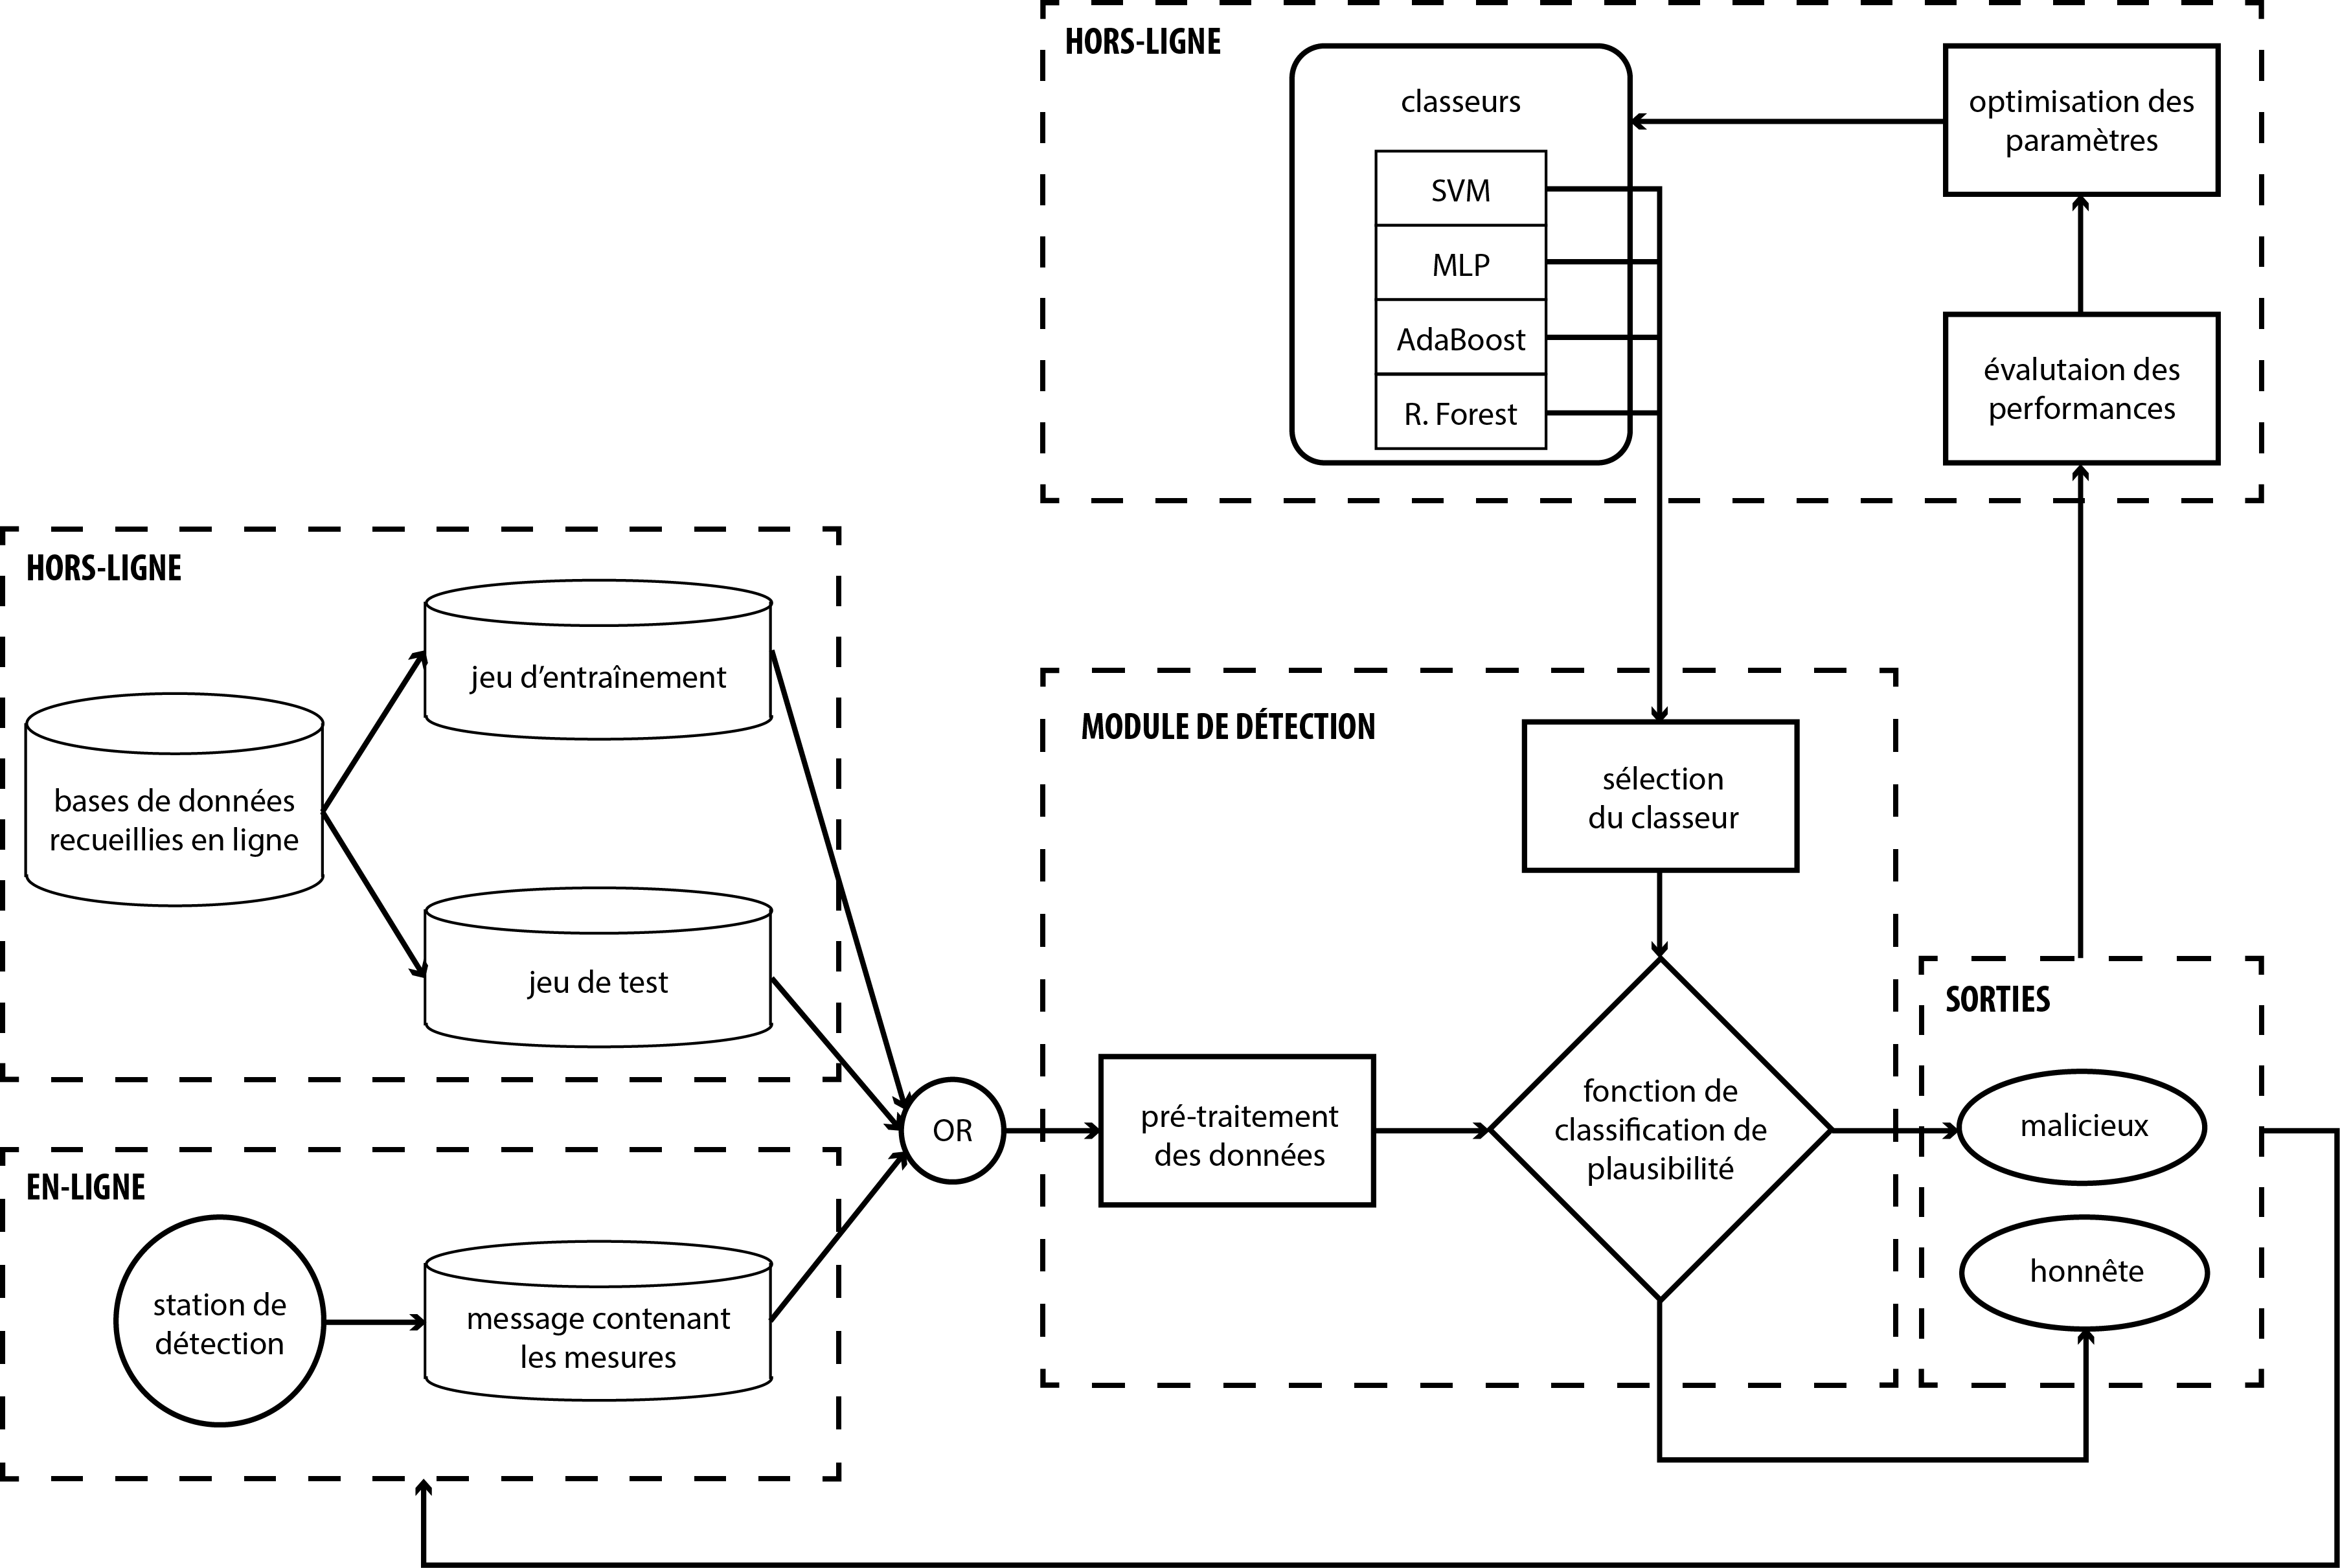
\includegraphics[width=.7\textwidth]{img/structure.png}
\caption{Structure du système de classification}
\end{figure}
\end{frame}

\begin{frame}{Système de classification}
\begin{description}
\item[A | Hors-ligne] Bases de données externes séparées en un jeu d'entraînement et un jeu de test
\item[B | En-ligne] Conception des messages à classer par les différents capteurs du véhicules
\item[C | Module de détection] Traitement des données et application de la fonction de classification
\item[D | Hors-ligne] Paramétrage et entraînement des classeurs ; évaluation des performances
\item[E | Sorties] Classes de sortie : message valide ou message malicieux
\end{description} 
\end{frame}

\section{Démarche de recherche}

\begin{frame}{Première implémentation}
\begin{itemize}
\item Extraction des colonnes largeur et longueur de la base de données
\item Suppression des redondances
\item Définition de zones de décision arbitraires
\item Génération des données malicieuses
\end{itemize}
\begin{table}
\centering
\begin{tabular}{llll}
validité & intervalle de longueur & intervalle de largeur \\
\hline
non-malicieux & 3 à 6,5 mètres & 1,4 à 2,4 mètres \\
malicieux & 3 à 4,1 mètres & 2,05 à 2,4 mètres \\
malicieux & 5,25 à 6,5 mètres & 1,4 à 1,65 mètres \\
\end{tabular}
\end{table}
\end{frame}

\begin{frame}{Première implémentation}
\begin{figure}
\centering
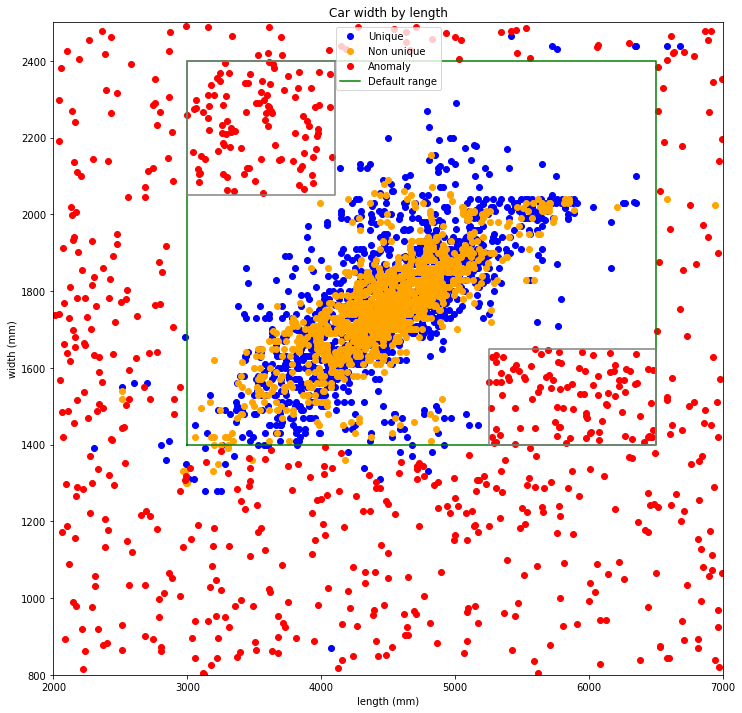
\includegraphics[width=.56\textwidth]{img/first_try.png}
\caption{Régions de décision arbitraires}
\end{figure}
\end{frame}

\begin{frame}{Chargement des bases de données}

\begin{enumerate}
\item Création de la matrice de classe : formatage des données issues des CSV
\item Création de la matrice globale en fusionnant les matrices de chaque classe
\item Instanciation de la classe \texttt{Dectector} \begin{enumerate}
\item Suppression des redondances
\item Génération des données malicieuses
\item Création du jeu d'entraînement et du jeu de test
\end{enumerate}
\end{enumerate}
\end{frame}

\begin{frame}{Chargement des bases de données}
\begin{figure}
\centering
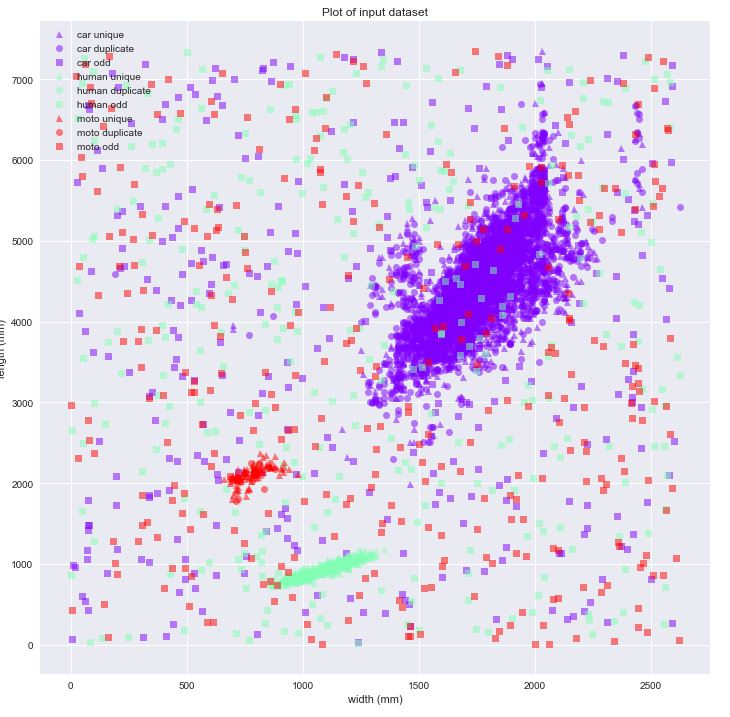
\includegraphics[width=.56\textwidth]{img/detector_plot.jpg}
\caption{Base de données après traitement}
\end{figure}
\end{frame}

\begin{frame}{Classe \texttt{Detector}}
\begin{itemize}
\item Pré-traitement \begin{itemize}
\item \texttt{clean}
\item \texttt{append\_odd\_points}
\item \texttt{format}
\end{itemize}
\item Interface scikit-learn \begin{itemize}
\item \texttt{classify}
\item \texttt{tune\_parameters}
\item \texttt{predict}
\end{itemize}
\item Affichage \begin{itemize}
\item \texttt{plot}
\item  \texttt{plot\_decision\_boudaries}
\end{itemize}
\end{itemize}
\end{frame}

\begin{frame}{Méthodes d'évaluation}
\framesubtitle{Matrice de confusion}

\begin{tabular}{ l | l | c | c | c c}
\multicolumn{2}{c}{} & \multicolumn{2}{c}{Classe réelle} & \\
\cline{3-4}
\multicolumn{2}{c|}{} & Positif & Négatif \\
\cline{2-4}
\multirow{2}{*}{Classe prédite} & Positif & $TP$ & $FP$ & $PPV$ & $FDR$ \\
\cline{2-4}
& Négatif & $FN$ & $TN$ & $FOR$ & $NPV$ \\
\cline{2-4}
\multicolumn{1}{r}{} & \multicolumn{1}{l}{} & \multicolumn{1}{c}{$TPR$} & \multicolumn{1}{c}{$FPR$} \\
\multicolumn{1}{l}{} & \multicolumn{1}{l}{} & \multicolumn{1}{c}{$FNR$} & \multicolumn{1}{c}{$TNR$} \\
\end{tabular}

\medskip

\begin{block}{Exemple pour Random Forest}
$$\begin{bmatrix}
2801 & 19 \\ 
36 & 467 \\
\end{bmatrix}$$
\end{block}

\end{frame}

\begin{frame}{Méthodes d'évaluation}
\framesubtitle{Différentes métriques}
\begin{itemize}
\item ratio de vrai positif: $TPR=\frac{TP}{TP+FN}=0.987$
\item ratio de vrai négatif: $TNR=\frac{TN}{TN+FP} = 0.959$
\item ratio de faux positif: $FPR=\frac{FP}{TP+TN}=0.04$
\item ratio de faux négatif: $FNR=\frac{FN}{TP+FN}=0.01 $
\item valeur prédictive positive: $PPV=\frac{TP}{TP+FP}=0.993$
\item valeur prédictive négative: $NPV=\frac{TN}{TN+FN}=0.928$
\item taux de fausses découvertes: $FDR=\frac{FP}{TP+FP}=0.001$
\item taux de fausses omissions: $FOR=\frac{FN}{TN+FN}=0.072$
\end{itemize}
\end{frame}

\begin{frame}{Méthodes d'évaluation}
\framesubtitle{Score F1}

\begin{block}{Objectif}
Maximisation du score F1 comme critère de performance
\end{block}

\begin{equation}
\text{f1-score} = \dfrac{2\times(\text{Recall} \times \text{Precision})}{(\text{Recall} + \text{Precision})} = 2\times\dfrac{PPV \times TPR}{PPV + TPR}
\end{equation}

\begin{equation}
\text{Precision} = \dfrac{TP}{TP+FP}
\end{equation}

\begin{equation}
\text{Recall} = \dfrac{TP}{TP+FN}
\end{equation}

\end{frame}

\section{Paramétrage et résultats}

\begin{frame}{Recherche exhaustive et validation croisée}
\begin{itemize}
\item Recherche des paramètres optimaux : \texttt{GridSearchCV}
\item Utilisation d'une fonction de score (F1-score) personnalisée
\item Export des données en formats exploitables (JSON, CSV) \begin{itemize}
\item Table des jeux de paramètres
\item Table des scores
\end{itemize}
\end{itemize}
\end{frame}

\begin{frame}{Paramètres optimaux}
\framesubtitle{Perceptron à couches multiples}

\begin{itemize}
\item Beaucoup de paramètres à tester (plus de 18 heures de test sur les serveurs InfRes)
\item Score F1 moyen maximal de 0.937
\item Beaucoup de fluctuations
\end{itemize}

\begin{table}
\centering
\begin{tabular}{l l l}
paramètre & rôle & valeur optimale \\
\hline
\texttt{learning\_rate} & taux d'apprentissage & \texttt{'constant'}\\
\texttt{alpha} & régularisation $l_2$ & $10^{-6}$ \\
\texttt{activation} & fonction d'activation & \texttt{'tanh'}\\
\texttt{solver} & descente du gradient & \texttt{'lbfgs'}\\
\texttt{hidden\_layer\_sizes} & couches cachées & \texttt{[28, 28, 28]}\\
\end{tabular}
\caption{Paramètres optimaux pour MLP}
\end{table}

\end{frame}

\begin{frame}
\begin{figure}
\centering
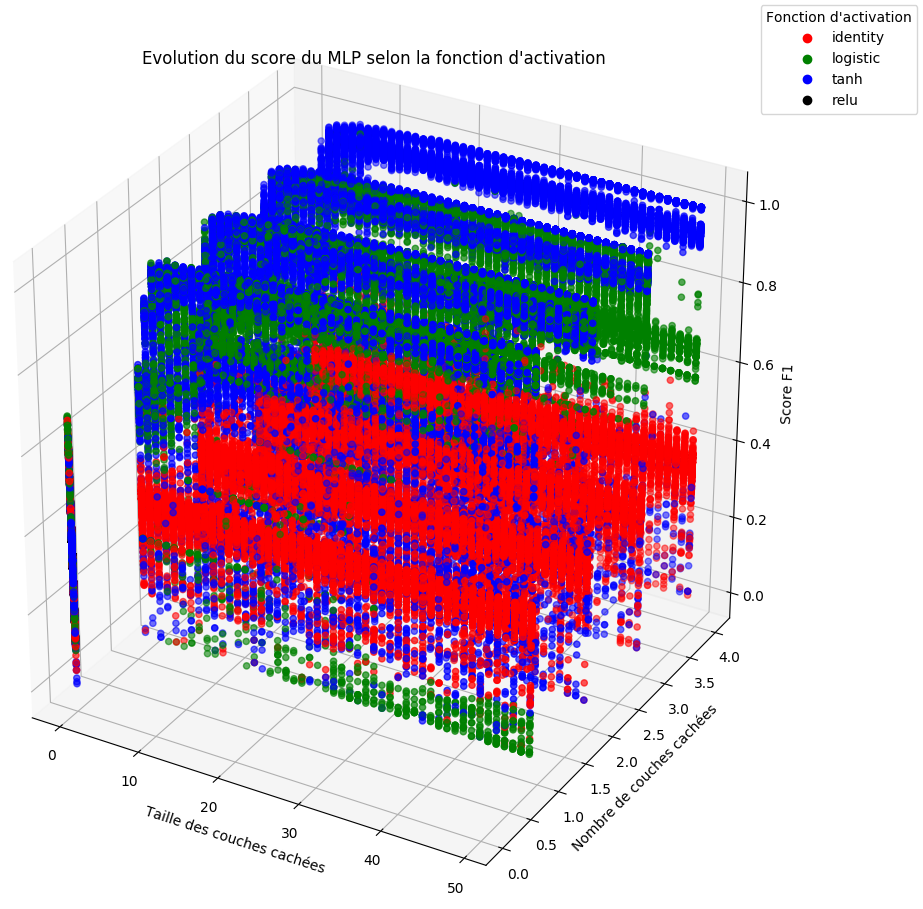
\includegraphics[width=.56\textwidth]{img/mlp_activation_crop.png}
\caption{Évolution du score du MLP selon la fonction d'activation}
\end{figure}
\end{frame}

\begin{frame}
\begin{figure}
\centering
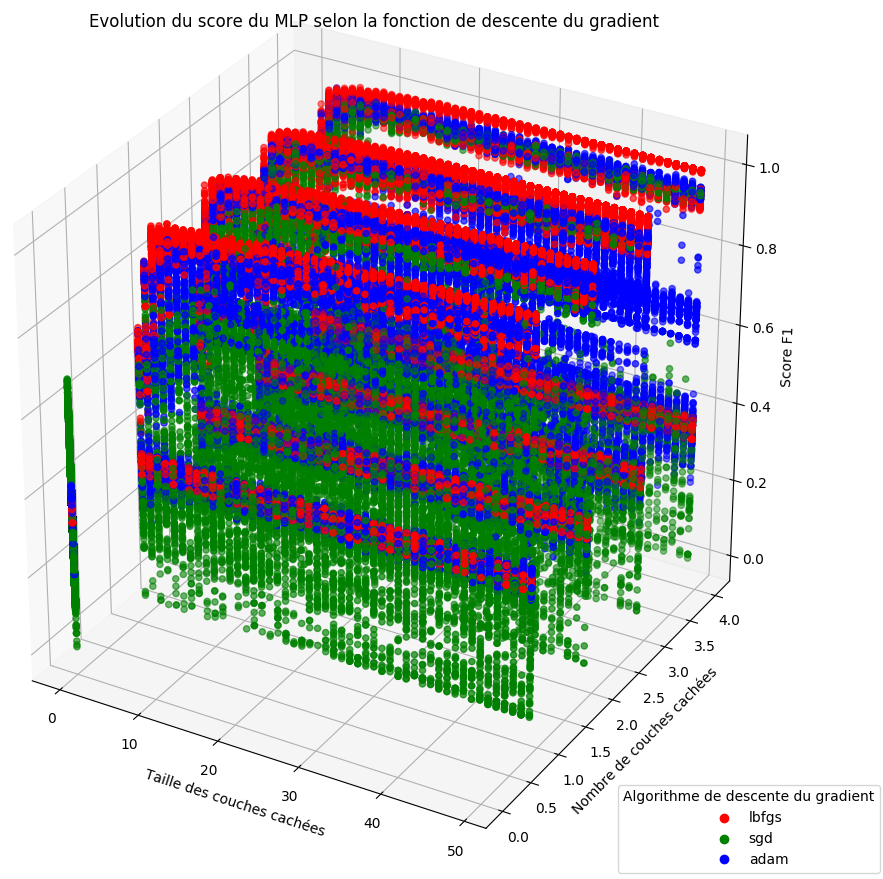
\includegraphics[width=.56\textwidth]{img/mlp_solver_crop.png}
\caption{Évolution du score du MLP selon l'algorithme de descente du gradient}
\end{figure}
\end{frame}

\begin{frame}{Paramètres optimaux}
\framesubtitle{AdaBoost}

\begin{itemize}
\item Tests relativement rapides
\item Scores rapidement bons (Score F1 moyen maximal de 0.947)
\item Beaucoup moins de fluctuations
\end{itemize}

\begin{table}
\centering
\begin{tabular}{l l}
paramètre & valeur optimale \\
\hline
\texttt{n\_estimators} & 46\\
\texttt{learning\_rate} & 0.3 \\
\texttt{base\_estimator} & Arbre de décision de profondeur maximale 3\\
\end{tabular}
\caption{Paramètres optimaux pour AdaBoost}
\end{table}

\end{frame}

\begin{frame}
\begin{figure}
\centering
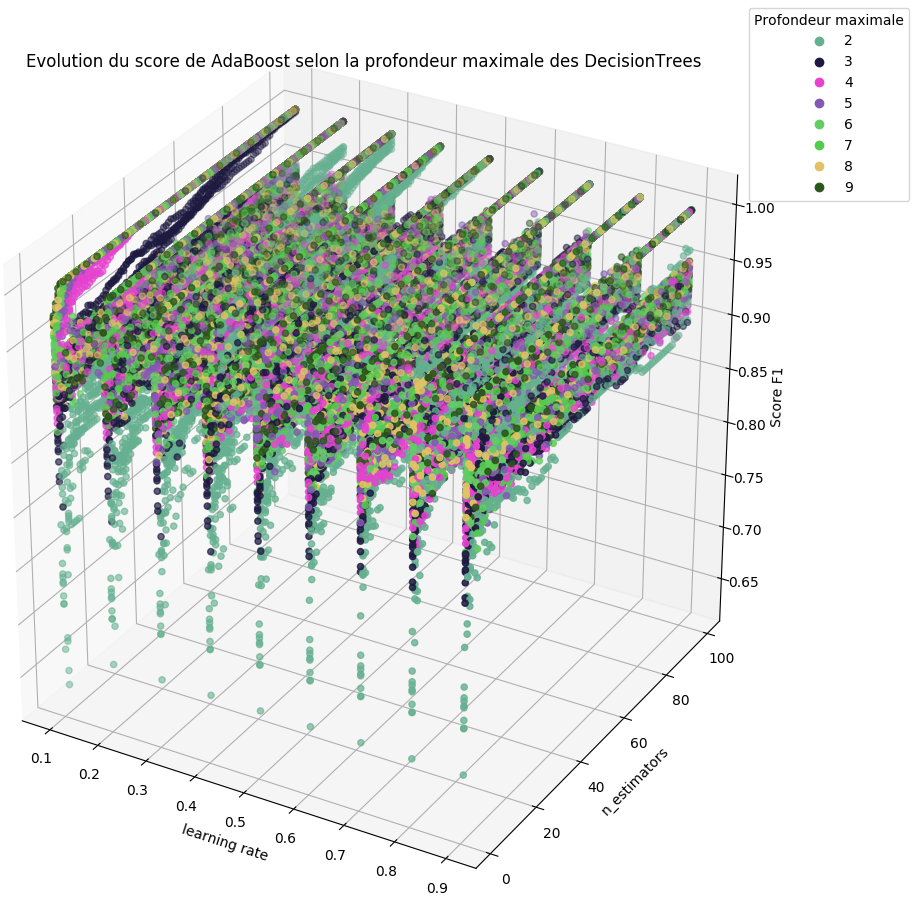
\includegraphics[width=.56\textwidth]{img/adaboost_depth.png}
\caption{Évolution du score de AdaBoost selon la profondeur maximale des DecisionTrees}
\end{figure}
\end{frame}


\begin{frame}{Problème multi-classe dans SVM}

Comparaison de deux méthodes d'adaptation au multiclasse :

\begin{itemize}
\item "One-Versus-the-Rest"
\item Méthode directe de Crammer et Singer
\end{itemize}

\begin{figure}
\centering
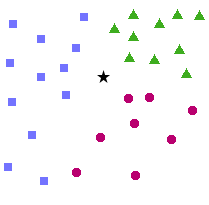
\includegraphics[scale=0.4]{img/svm.png} \hspace{2pt}

\includegraphics[scale=0.4]{img/svm_OneVsAll.png}
\caption{Problème multi-classe et séparation "One-Versus-the-Rest"\label{fig:one_versus_rest}}
\end{figure}

\end{frame}


\begin{frame}{Paramètres optimaux}
\framesubtitle{SVM}

\begin{itemize}
\item Très long temps de calcul
\item Score F1 moyen maximal de 0.934
\end{itemize}

\begin{table}
\centering
\begin{tabular}{lll}
paramètre & valeurs testées & valeurs optimales \\
\hline
\texttt{multi\_class} & \texttt{ovr}, \texttt{crammer\_singer} & \texttt{crammer\_singer} \\
\texttt{C} & $\{10^k \>\> | \>\> k \in [\![-2, 3]\!] \}$ & 100 \\
\texttt{tol} & $\{10^{-k} \>\> | \>\> k \in [\![3, 6]\!] \}$ & 0.00001 \\
\end{tabular}
\caption{Paramètres testés et paramètres optimaux pour SVM}
\end{table}

\end{frame}

\begin{frame}{Performances des classeurs}
\begin{table}
\centering
\begin{tabular}{r | llllll}
& \emph{TPR} & \emph{FPR} & \emph{TNR} & \emph{FNR} & \emph{PPV} & \emph{f1-score} \\ 
MLP & 0.568 & 0.005 & 0.995 & 0.432 & 0.949 & 0.711 \\
AdaBoost & 0.935 & 0.010 & 0.990 & 0.065 & 0.941 & 0.938 \\
SVM & 0.966 & 1.0 & 0.0 & 0.034 & 0.145 & 0.252 \\
R. Forest & 0.917 & 0.007 & 0.993 & 0.083 & 0.960 & 0.938 \\
\end{tabular}
\caption{Détails des scores en fonction des classeurs après paramétrage}
\end{table}

\begin{itemize}
\item AdaBoost et Random Forest se démarquent
\item SVM reste très décevant
\end{itemize}

\end{frame}

\begin{frame}{Régions de décision}
\begin{figure}
\centering
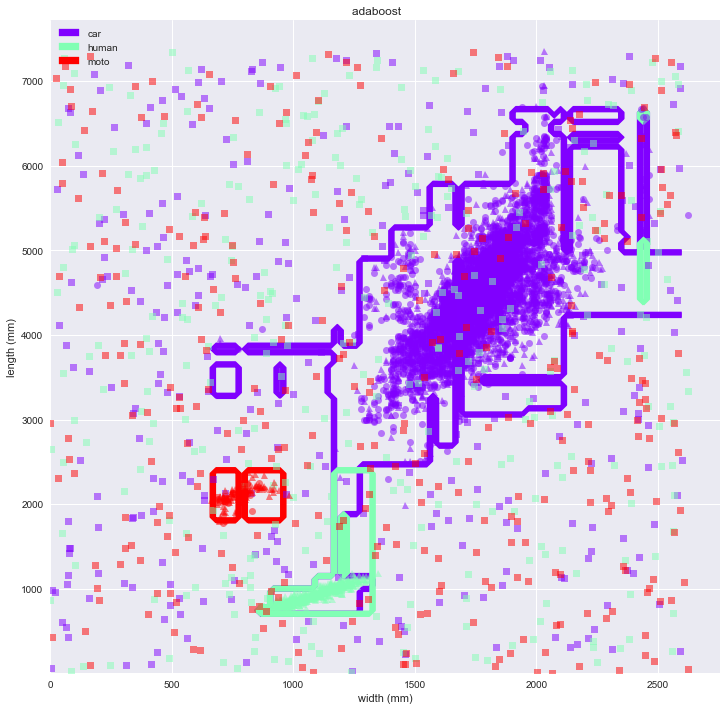
\includegraphics[width=.58\textwidth]{img/adaboost_contour.png}
\caption{Régions de décisions pour le classeur AdaBoost}
\end{figure}
\end{frame}

\begin{frame}{Prédiction en ligne}
\begin{enumerate}
\item Créer un objet \texttt{Detector} en chargeant les bases de données récoltées
\item Entraîner un classeur, dont les paramètres sont ceux résultant de l'optimisation effectuée précédemment, avec ces données
\item Attribuer ce classeur en tant que classeur de prédiction pour le \texttt{Detector}
\item Sauvegarder la méthode \texttt{predict}
\end{enumerate}
\end{frame}

\section{Conclusion}
\begin{frame}{Conclusion}

Dans ce travail, nous avons:
\begin{itemize}

\item implémenté un algorithme de classification d’obstacles,

\item mené une étude de comparative de performances selon le score F1

\end{itemize} 

\medskip
\begin{block}{Résultats}
Les algorithmes de Random Forest et AdaBoost atteignent des score F1 supérieurs à 0.93
\end{block}


\begin{block}{Travaux futurs}
Orienter les recherches sur la sécurité du dispositif
\end{block}


\end{frame}

\begin{frame}
\begin{center}

\begin{Huge}
\color{Blue}Merci pour votre attention.
\end{Huge}
\end{center}
\end{frame}

\end{document}
